The error discussed in \secref{sec:simpleExample} can be remedied in many ways. One way is by changing the workflow to initially negotiate \emph{price} and \emph{terms} separately. This change is shown in \figref{fig:face2face_workflow_fixed}. In the new workflow, only one of either \emph{price} or \emph{terms} changes at a time, making it impossible to transition directly from \emph{Init Purchase Pending} to \emph{Purchase Agreed}.

This problem could also be addressed by altering the CWP in a way that makes negotiations optional. Adding a transition from \emph{Init Purchase Pending} to \emph{Purchase Agreed} is a straightforward way of doing that.

\begin{figure*}[t]
  \begin{center}
    \begin{tabular}{c}
        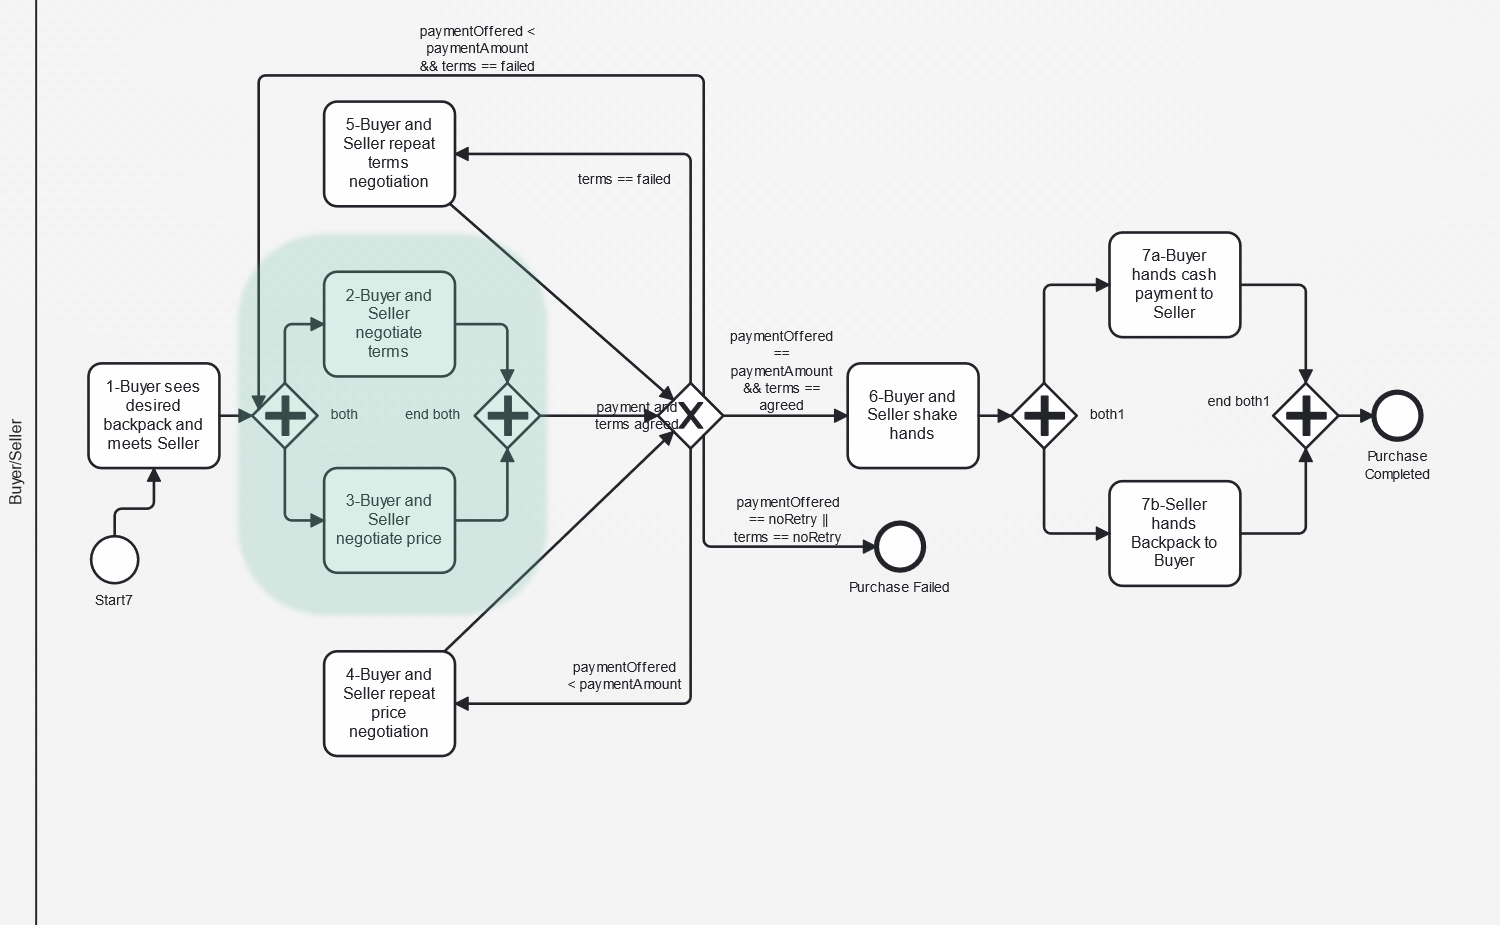
\includegraphics[width=\textwidth]{../figs/BPMN/face2face_May_5_2023_workflow_fixed.png}
    \end{tabular}
  \end{center}
\caption{Fixed BPMN Workflow for \facetoface}
\label{fig:face2face_workflow_fixed}
\end{figure*}

\figref{fig:buynsell_bpmn} shows the BPMN of a remote purchase system named \buynsell. This BPMN model is similar to \facetoface~except that it splits the buyer and seller into different parties, as well as introduces some reasoning about fulfillment of the order. \buynsell shares a CWP with the previous example, shown in \figref{fig:PurchaseCWP}. This example was chosen partially to show the versatility of CWP. Because it shouldn't reason at all about the context or the actors in the work, it can be used to verify multiple BPMN diagrams involving an exchange of goods, even though they may have drastically different performance characteristics. Additionally, this example introduces asynchrony by dividing the work between two actors in separate swimlanes. This asynchrony is where manual reasoning becomes more difficult, and where the value of model checking becomes more apparent.

\begin{figure*}[t]
  \begin{center}
    \begin{tabular}{c}
        \includesvg[inkscapeformat=png, width=\textwidth]{../figs/BPMN/buynsell_Mar_27_2023_workflow.svg}
    \end{tabular}
  \end{center}
\caption{BPMN workflow for remote purchase example, \buynsell}
\label{fig:buynsell_bpmn}
\end{figure*}

\figref{fig:phware_bpmn} shows the BPMN of the original example from \cite{mercer22}. In this example, a patient diagnosed with COVID-19 is being monitored remotely. \figref{fig:phware_cwp} shows the corresponding CWP. When we verify the BPMN against this CWP, we are ensuring that the patient is never incidentally mistreated in the BPMN according to the readings from the remote monitoring device. The initial example shows a single actor with branching paths. The second example shows multiple actors with mostly linear paths. This is the most complicated example so far, containing both multiple actors and branching paths.

\begin{figure*}[t]
  \begin{center}
    \begin{tabular}{c}
        \includesvg[inkscapeformat=png, width=\textwidth]{../figs/BPMN/phware_May_5_workflow.svg}
    \end{tabular}
  \end{center}
\caption{BPMN workflow for \phware~example}
\label{fig:phware_bpmn}
\end{figure*}

\begin{figure*}[t]
  \begin{center}
    \begin{tabular}{c}
        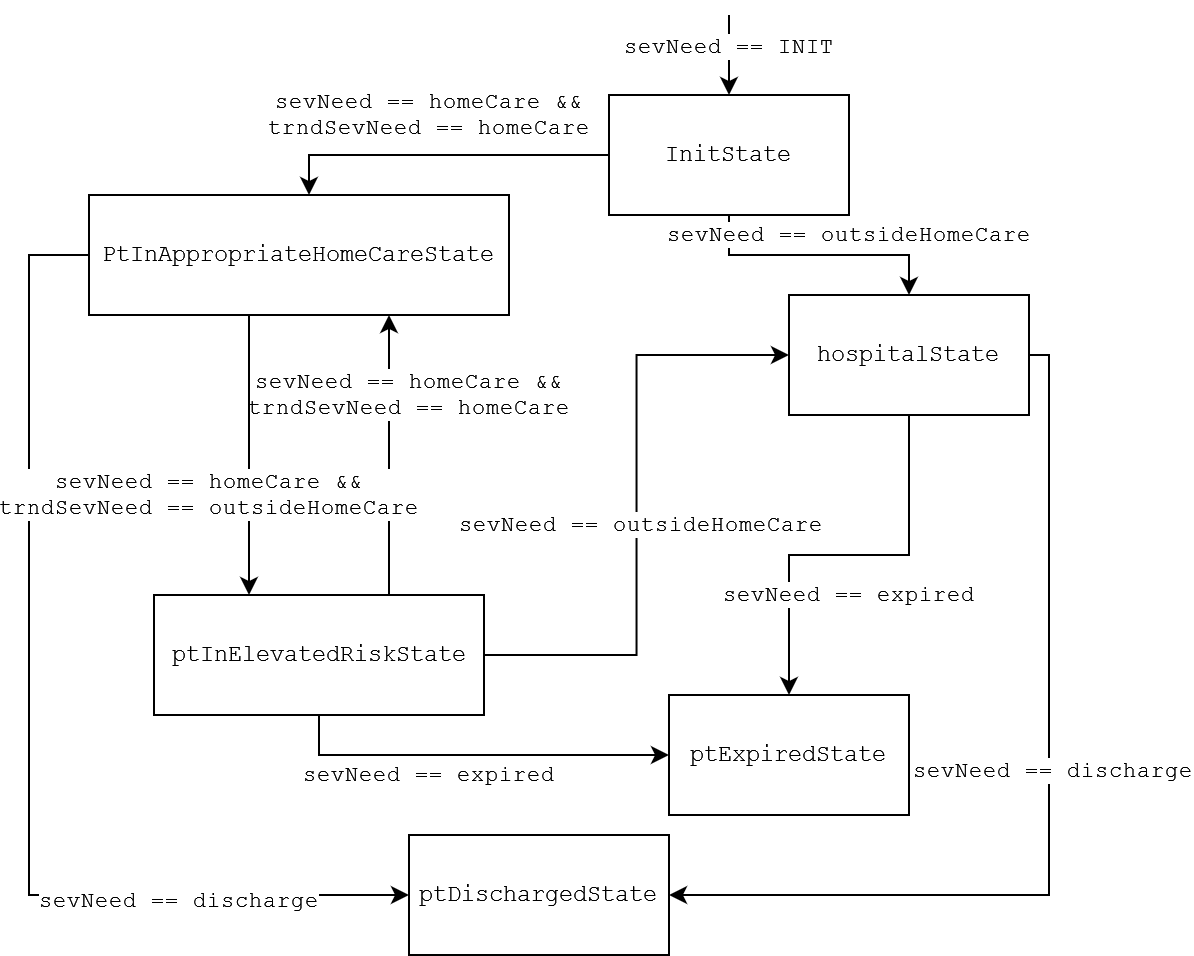
\includegraphics[width=\textwidth]{../figs/CWP/phware_CWP.png}
    \end{tabular}
  \end{center}
\caption{CWP state diagram for \phware~example}
\label{fig:phware_cwp}
\end{figure*}

\figref{fig:ParallelScaling} shows a general version of the sequential scaling example BPMN and CWP. In this example, we show the scalability of the automation and verification process. This example contains a single actor with multiple decisions to make sequentially.
This number of decisions can be increased to push the limits of model checking in this context. The CWP here has just two states, only requiring that the BPMN execute to completion.


\figref{fig:SequentialScaling} shows the BPMN and CWP of the parallel scaling example. This is also an example to show scalability. In this example, there are multiple actors, each with a single decision to make. It is important to note that all of the actors interact with a single global state variable here. The CWP used in this example is identical to the sequential scaling example.

\begin{figure*}[t]
  \begin{center}
    \begin{tabular}{c}
        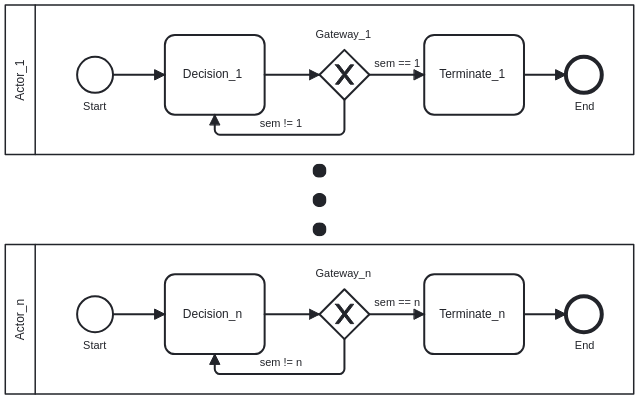
\includegraphics[width=\textwidth]{../figs/BPMN/ParallelScalingWorkflow.png} \\ 
        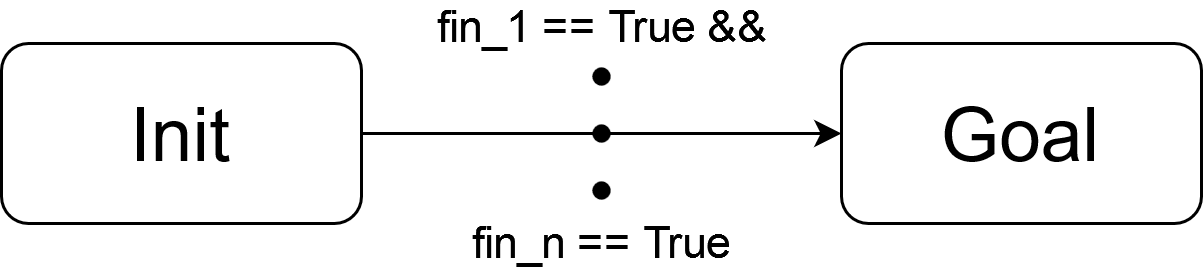
\includegraphics[width=\textwidth]{../figs/CWP/general_scaling_cwp.png}
    \end{tabular}
  \end{center}
\caption{BPMN workflow for parallel scaling with n actors}
\label{fig:ParallelScaling}
\end{figure*}


\begin{figure*}[t]
  \begin{center}
    \begin{tabular}{c}
        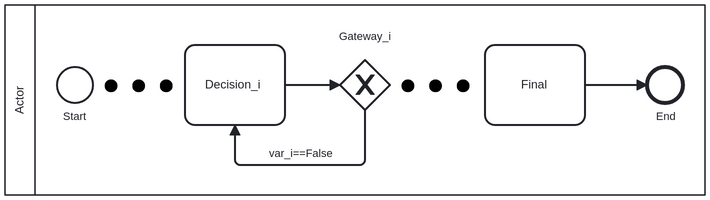
\includegraphics[width=\textwidth]{../figs/BPMN/SequentialScalingWorkflow.png} \\
        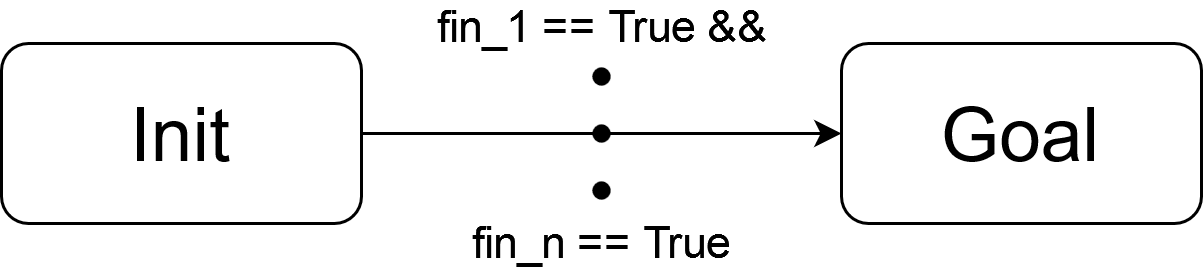
\includegraphics[width=\textwidth]{../figs/CWP/general_scaling_cwp.png}
    \end{tabular}
  \end{center}
\caption{BPMN workflow for sequential scaling}
\label{fig:SequentialScaling}
\end{figure*}
